\chapter{Introduction au Big Data}
	
	\section{Introduction}
	
	Big Data est un terme associé aux données massives, rapidement générées, ayant une grande diversité où les  outils traditionnels sont incapables de gérer ces données. La complexité du Big Data vient du fait que tout type de données peut être utilisé, en vue de livrer la bonne information à la bonne personne et au bon moment afin d'aider à prendre les bonnes décisions.
	
	
	\section{Quelques concepts associés au Big Data}
		\subsection{Définition du Big Data : Volume, Vélocité, Variété et Véracité}
		
		IBM définit Big Data suivant les quatre dimensions suivants : volume, variété, vélocité et véracité. 
		\paragraph{Volume de données}~
		La quantité de données manipulées par les outils traditionnels de la gestion des données est de l'ordre de Gigaoctets (GB) et de Téraoctets (TB). Toutefois, le Big Data est mesuré en Pétaoctets (PB) et Exaoctets (EB). Une des premières applications du Big Data est la recherche dans Word-Wide Web (WWW). Selon une étude (\cite{6567202}, $2013$) de l'International Data Corporation (IDC), le volume de données  va atteindre $40$ Zettaoctets\footnote{ $ 1 ZB = 1000000000000 GB $} par  entreprise en $2020$ .
		
		\paragraph{Vélocité de données} ~
		le Big Data est généré à travers des milliards
		d'appareils, ces données générées sont communiquées avec la vitesse de la lumière à travers l'Internet. L'augmentation de la vitesse de l'Internet est une  des raisons ayant favorisé l'augmentation de la vitesse de la génération des données.	
		%la vitesse décrit la fréquence de la génération et du partage des données. Autrement dit, les données sont générées rapidement et doivent être traitées rapidement pour extraire les informations  pertinentes.
		Par exemple, Wallmart (international discount retail chain) génère environ   $2.5$ Pétaoctets de données chaque  heure via les transactions de ses consommateurs\footnote{Source : \url{https://www.bernardmarr.com/default.asp?contentID=690}, consultée le $ 30/06/2018 $.}.
		
		
		
		
		
		\paragraph{Variété de données} \label{variete-data}
		
		Le Big Data inclut toutes les formes des données, des fonctions diversifiés des données et des sources multiples des données.
		
		Le premier aspect de la variété  des données massives est la \textbf{forme} de celles-ci, les données manipulées incluent du texte, des graphes, des cartes, des vidéos, des photos, etc.
		
		Le deuxième aspect de la variété des données massives concerne les \textbf{fonctions} assurées par ces données. Des données sont issues des conversations humaines, d'autres des transactions des consommateurs, ou bien des données archivées, etc.
		
		La source du Big Data est le troisième aspect de la variété. Des données sont en provenance des téléphones mobiles, des tablettes ou des ordinateurs portables, des fichiers journaux, du réseau de capteurs, etc. Les sources du Big Data peuvent être classées en trois grandes catégories : communications \textbf{\textit{human to human}} comme les conversations échangées dans les réseaux sociaux, communications \textbf{\textit{ human to machine}} comme l'accès des utilisateurs aux données dans le web et enfin communications \textbf{\textit{machine to machine}} comme les données issues de la communication entre les capteurs dans un réseau de capteurs.
		%au-delà des données des transactions habituelles des consommateurs, les données manipulées sont en provenance de sources différentes et de formats différents. Par exemple: des vidéos, des documents, des commentaires, des données géospatiales, des journaux, etc. Les grands ensembles de données sont constitués de données structurées et non structurées, publiques ou privées, locales ou distantes, partagées ou confidentielles, complètes ou incomplètes, etc.
		
		
		
		\paragraph{Véracité de données}
		
		La véracité concerne la crédibilité et la qualité des données. La mauvaise qualité de données est due à de nombreuses raisons telles que les pannes techniques comme le dysfonctionnement des appareils comme les capteurs, les erreurs humaines,  etc. De plus, les données peuvent être intentionnellement erronées pour des raisons de concurrence ou des raisons stratégiques.
	
		\subsection{Une architecture du Big Data}
		
		L'architecture présentée dans ce qui suit est celle proposée dans  \cite{anil-big-data}, elle est illustrée dans la figure \ref{fig:bigdata-architecture}.
		
		Il existe plusieurs sources de données. Ces données  passent ensuite par \textit{ingest system}. Ensuite, les données peuvent passer par deux systèmes : un \textit{stream processing } et un \textit{batch processing}.  Les résultats de ce traitement peuvent être envoyées vers les bases de données NoSQL pour une utilisation ultérieure, ou bien  utiliser ces résultats comme entrées pour d'autres applications. Ainsi, une solution Big Data comprend typiquement  ces  couches logiques. Chacune des couches peut être représentée par une ou plusieurs technologies disponibles. Reprenant chacune des composantes logiques:
		
		
		
		\paragraph{Big Data sources layer} Le choix des sources de donnés pour une application donnée dépend des objectifs qui dirigent l'analyse en question. Les sources avec leurs différents aspects sont détaillées dans la section \ref{variete-data}.
		
		\paragraph{Data Ingest layer} Cette couche permet de récupérer les données depuis les différentes sources de données. Ainsi, les données sont accueillies à travers des points d'entrées multiples. Ces points  sont capables d'acquérir ces données ayant une vélocité variable ainsi qu'une quantité aussi variable.  Après avoir traversé  \textit{Data Ingest layer}, les données sont envoyées au \textit{batch processing system}, au \textit{realtime processing system}, ou bien à un système de stockage particulier.
		
		\paragraph{Batch processing layer} Les données reçues sont celles en provenance du \textit{Data Ingest} ou bien d'une des bases de données NoSQL. Ces données sont ensuite traitées en utilisant les techniques de la programmation parallèle, en vue de fournir les résultats souhaités. La présente couche doit avoir connaissance des sources de données, les types de données, les algorithmes qui vont travailler sur ces données et enfin les résultats souhaités. Les résultats des traitements peuvent être utilisées par une des applications ou bien sauvegarder ces données dans une des bases de données adaptées.
		
		
		\paragraph{Stream Processing layer} Cette couche approvisionne les données directement d'une des entrées du \textit{Data Ingest layer}. Pareillement  à  \textit{Batch processing layer} en matière  des techniques de la programmation parallèle utilisées ainsi que la nécessité d'avoir les détails sur les sources des données, les types de données et les résultats souhaités.
		
		
		\paragraph{Data organizing layer} Le rôle de cette couche est d'organiser les données afin de faciliter l'accès à ces dernières. Ce sont les  données obtenues  de la part de la  couche  \textit{Stream Processing} ainsi que la couche \textit{Batch processing}. Cette couche est représentée par les bases de données NoSQL. Il existe plusieurs catégories de bases de données NoSQL.
		
		\paragraph{Infrastructure layer} Cette composante est responsable de la gestion des ressources de stockage, les ressources du calcul et la gestion de la communication. 
		Les fonctionnalités de cette couche sont fournies à travers le cloud computing.
		
		\paragraph{Distributed File System Layer} Cette couche assure le stockage d'une grande quantité de données, de sorte que ces données soient rapidement et facilement accessibles à toute les couches qui forment un système du Big Data. C'est ce que assure Hadoop Distributed File System (HDFS).
		
		\paragraph{Data consumption} Cette dernière couche utilise les sorties produits par les couches de l'analyse. Les résultats fournis peuvent être sous format de rapport, des dashboards, des visualisations, un moteur de recommandation ou tout autre format.
		
		
		
		
		
	
		\begin{figure}[H]
			\captionsetup{justification = centering}
			\centering
			\includegraphics[width=1\linewidth]{illustrations/bigdata-architecture}
			\caption{Architecture générique du Big Data \cite{anil-big-data}}
			\label{fig:bigdata-architecture}
			
		\end{figure}

	
	\subsection{Les bases de données NoSQL (Not Only SQL) } \label{sec:nosql}
	
	
	\paragraph{Introduction } ~
	
    Au cours de ces dernières années, on constate une révolution dans le stockage de données non structurées ayant une taille importante.  Car les objets à sauvegarder sont complexes; ils sont issus de sources hétérogènes.  Cette complexité a mis en question les performances des bases de données relationnelles. 
	
	Le terme NoSQL est apparu pour la première fois en $ 1998 $. Carlo Strozzi  a parlé des bases de données relationnelles qui n'utilisent pas le SQL comme langage d'interrogation des tables. Des années plus tard, des solutions  open source basées sur ce concept ont vu le jour. 
	
	Les bases de données relationnelles sont utilisées par la majorité des entreprises pour plusieurs raisons :   la facilité d'utilisation, la disponibilité de plusieurs produits et développeurs, etc. Ces dernières années, avec l'augmentation exponentielle de la quantité de données générées par certaines entreprises, ces dernières ont constaté l'insuffisance des Systèmes de Gestion de Bases de Données Relationnelles (SGBDR) pour répondre à leurs besoins.
	
    %	\paragraph{ Les besoins auxquels répondent NoSQL}  ~
	
	Les bases de données NoSQL sont conçues pour gérer des  volumes de données importants. L'idée de base de ces bases, c'est d'abord assurer la capacité de stocker des données de grande échelle dont leur  quantité  évolue rapidement, voire exponentiellement.  En deuxième lieu, les données stockées  doivent être interrogées  avec efficacité. Les données stockées dans  les bases de données NoSQL n'obéissent pas à un modèle prédéfini comme le cas des bases de données relationnelles. Cette flexibilité est une des caractéristiques des bases de données NoSQL.
	
	
	\paragraph{Types de base de données NoSQL} \label{sec:nosql-database}  ~
	
	Il existe quatre catégories distinctes de bases de données NoSQL. Chaque catégorie répond  à des besoins particuliers. Ainsi, on distingue les bases de données clé-valeur, document, graphe et colonne.
	
	


	\subparagraph {Clé-valeur} Une base de données de type clé-valeur repose sur le paradigme clé-valeur; chaque donnée, que ce soit un nombre, du texte ou tout autre élément est associé à une clé unique. Cette clé est le seul moyen d'accéder aux données stockées.
	Dans les bases de données NoSQL de type clé-valeur, les enregistrements  n'adhèrent pas à une structure prédéfinie. Par exemple, on peut avoir le premier enregistrement de type entier et le deuxième enregistrement de type texte. Cela assure une forte évolutivité grâce à l'absence d'une structure ou de typage. La figure \ref{fig:key-value-nosql} reprend un exemple d'une base de données NoSQL de type clé-valeur.

	
	\begin{figure}[H]
		\captionsetup{justification=centering}
		\centering
		\resizebox{!}{!}{
			% Graphic for TeX using PGF
% Title: /home/hayat/report_memoire/illustrations/key-value-nosql.dia
% Creator: Dia v0.97+git
% CreationDate: Sun Dec  2 15:37:59 2018
% For: hayat
% \usepackage{tikz}
% The following commands are not supported in PSTricks at present
% We define them conditionally, so when they are implemented,
% this pgf file will use them.
\ifx\du\undefined
  \newlength{\du}
\fi
\setlength{\du}{15\unitlength}
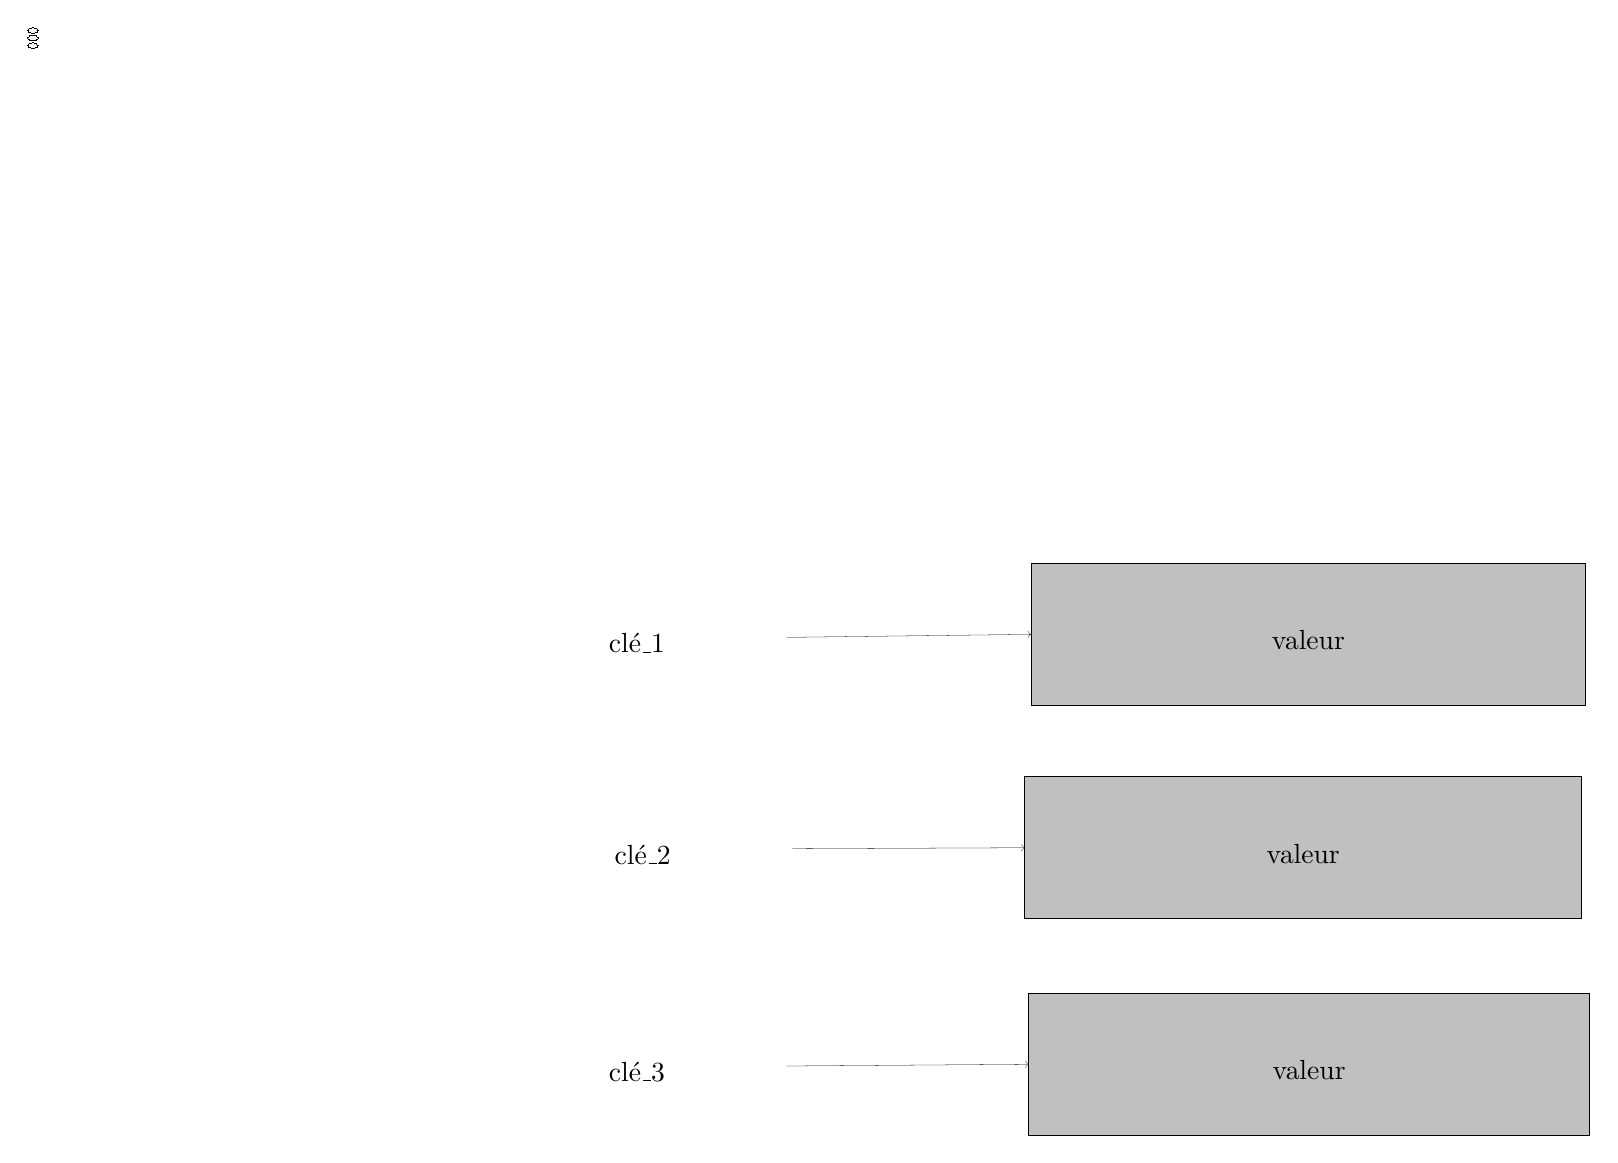
\begin{tikzpicture}[even odd rule]
\pgftransformxscale{1.000000}
\pgftransformyscale{-1.000000}
\definecolor{dialinecolor}{rgb}{0.000000, 0.000000, 0.000000}
\pgfsetstrokecolor{dialinecolor}
\pgfsetstrokeopacity{1.000000}
\definecolor{diafillcolor}{rgb}{1.000000, 1.000000, 1.000000}
\pgfsetfillcolor{diafillcolor}
\pgfsetfillopacity{1.000000}
\pgfsetlinewidth{0.000000\du}
\pgfsetdash{}{0pt}
\pgfsetmiterjoin
\definecolor{diafillcolor}{rgb}{0.960784, 0.960784, 0.960784}
\pgfsetfillcolor{diafillcolor}
\pgfsetfillopacity{1.000000}
\pgfpathellipse{\pgfpoint{7.950991\du}{7.987995\du}}{\pgfpoint{1.899011\du}{0\du}}{\pgfpoint{0\du}{1.012005\du}}
\pgfusepath{fill}
\definecolor{dialinecolor}{rgb}{0.000000, 0.000000, 0.000000}
\pgfsetstrokecolor{dialinecolor}
\pgfsetstrokeopacity{1.000000}
\pgfpathellipse{\pgfpoint{7.950991\du}{7.987995\du}}{\pgfpoint{1.899011\du}{0\du}}{\pgfpoint{0\du}{1.012005\du}}
\pgfusepath{stroke}
% setfont left to latex
\definecolor{dialinecolor}{rgb}{0.000000, 0.000000, 0.000000}
\pgfsetstrokecolor{dialinecolor}
\pgfsetstrokeopacity{1.000000}
\definecolor{diafillcolor}{rgb}{0.000000, 0.000000, 0.000000}
\pgfsetfillcolor{diafillcolor}
\pgfsetfillopacity{1.000000}
\node[anchor=base,inner sep=0pt, outer sep=0pt,color=dialinecolor] at (7.950991\du,8.182995\du){clé\_1};
\pgfsetlinewidth{0.000000\du}
\pgfsetdash{}{0pt}
\pgfsetmiterjoin
\definecolor{diafillcolor}{rgb}{0.960784, 0.960784, 0.960784}
\pgfsetfillcolor{diafillcolor}
\pgfsetfillopacity{1.000000}
\pgfpathellipse{\pgfpoint{8.024011\du}{10.672005\du}}{\pgfpoint{1.899011\du}{0\du}}{\pgfpoint{0\du}{1.012005\du}}
\pgfusepath{fill}
\definecolor{dialinecolor}{rgb}{0.000000, 0.000000, 0.000000}
\pgfsetstrokecolor{dialinecolor}
\pgfsetstrokeopacity{1.000000}
\pgfpathellipse{\pgfpoint{8.024011\du}{10.672005\du}}{\pgfpoint{1.899011\du}{0\du}}{\pgfpoint{0\du}{1.012005\du}}
\pgfusepath{stroke}
% setfont left to latex
\definecolor{dialinecolor}{rgb}{0.000000, 0.000000, 0.000000}
\pgfsetstrokecolor{dialinecolor}
\pgfsetstrokeopacity{1.000000}
\definecolor{diafillcolor}{rgb}{0.000000, 0.000000, 0.000000}
\pgfsetfillcolor{diafillcolor}
\pgfsetfillopacity{1.000000}
\node[anchor=base,inner sep=0pt, outer sep=0pt,color=dialinecolor] at (8.024011\du,10.867005\du){clé\_2};
\pgfsetlinewidth{0.000000\du}
\pgfsetdash{}{0pt}
\pgfsetmiterjoin
\definecolor{diafillcolor}{rgb}{0.960784, 0.960784, 0.960784}
\pgfsetfillcolor{diafillcolor}
\pgfsetfillopacity{1.000000}
\pgfpathellipse{\pgfpoint{7.949011\du}{13.432005\du}}{\pgfpoint{1.899011\du}{0\du}}{\pgfpoint{0\du}{1.012005\du}}
\pgfusepath{fill}
\definecolor{dialinecolor}{rgb}{0.000000, 0.000000, 0.000000}
\pgfsetstrokecolor{dialinecolor}
\pgfsetstrokeopacity{1.000000}
\pgfpathellipse{\pgfpoint{7.949011\du}{13.432005\du}}{\pgfpoint{1.899011\du}{0\du}}{\pgfpoint{0\du}{1.012005\du}}
\pgfusepath{stroke}
% setfont left to latex
\definecolor{dialinecolor}{rgb}{0.000000, 0.000000, 0.000000}
\pgfsetstrokecolor{dialinecolor}
\pgfsetstrokeopacity{1.000000}
\definecolor{diafillcolor}{rgb}{0.000000, 0.000000, 0.000000}
\pgfsetfillcolor{diafillcolor}
\pgfsetfillopacity{1.000000}
\node[anchor=base,inner sep=0pt, outer sep=0pt,color=dialinecolor] at (7.949011\du,13.627005\du){clé\_3};
\pgfsetlinewidth{0.000000\du}
\pgfsetdash{}{0pt}
\pgfsetmiterjoin
{\pgfsetcornersarced{\pgfpoint{0.000000\du}{0.000000\du}}\definecolor{diafillcolor}{rgb}{0.752941, 0.752941, 0.752941}
\pgfsetfillcolor{diafillcolor}
\pgfsetfillopacity{1.000000}
\fill (12.956200\du,7.050000\du)--(12.956200\du,8.850000\du)--(19.999950\du,8.850000\du)--(19.999950\du,7.050000\du)--cycle;
}{\pgfsetcornersarced{\pgfpoint{0.000000\du}{0.000000\du}}\definecolor{dialinecolor}{rgb}{0.000000, 0.000000, 0.000000}
\pgfsetstrokecolor{dialinecolor}
\pgfsetstrokeopacity{1.000000}
\draw (12.956200\du,7.050000\du)--(12.956200\du,8.850000\du)--(19.999950\du,8.850000\du)--(19.999950\du,7.050000\du)--cycle;
}% setfont left to latex
\definecolor{dialinecolor}{rgb}{0.000000, 0.000000, 0.000000}
\pgfsetstrokecolor{dialinecolor}
\pgfsetstrokeopacity{1.000000}
\definecolor{diafillcolor}{rgb}{0.000000, 0.000000, 0.000000}
\pgfsetfillcolor{diafillcolor}
\pgfsetfillopacity{1.000000}
\node[anchor=base,inner sep=0pt, outer sep=0pt,color=dialinecolor] at (16.478075\du,8.145000\du){valeur};
\pgfsetlinewidth{0.000000\du}
\pgfsetdash{}{0pt}
\pgfsetmiterjoin
{\pgfsetcornersarced{\pgfpoint{0.000000\du}{0.000000\du}}\definecolor{diafillcolor}{rgb}{0.752941, 0.752941, 0.752941}
\pgfsetfillcolor{diafillcolor}
\pgfsetfillopacity{1.000000}
\fill (12.875000\du,9.760000\du)--(12.875000\du,11.560000\du)--(19.950000\du,11.560000\du)--(19.950000\du,9.760000\du)--cycle;
}{\pgfsetcornersarced{\pgfpoint{0.000000\du}{0.000000\du}}\definecolor{dialinecolor}{rgb}{0.000000, 0.000000, 0.000000}
\pgfsetstrokecolor{dialinecolor}
\pgfsetstrokeopacity{1.000000}
\draw (12.875000\du,9.760000\du)--(12.875000\du,11.560000\du)--(19.950000\du,11.560000\du)--(19.950000\du,9.760000\du)--cycle;
}% setfont left to latex
\definecolor{dialinecolor}{rgb}{0.000000, 0.000000, 0.000000}
\pgfsetstrokecolor{dialinecolor}
\pgfsetstrokeopacity{1.000000}
\definecolor{diafillcolor}{rgb}{0.000000, 0.000000, 0.000000}
\pgfsetfillcolor{diafillcolor}
\pgfsetfillopacity{1.000000}
\node[anchor=base,inner sep=0pt, outer sep=0pt,color=dialinecolor] at (16.412500\du,10.855000\du){valeur};
\pgfsetlinewidth{0.000000\du}
\pgfsetdash{}{0pt}
\pgfsetmiterjoin
{\pgfsetcornersarced{\pgfpoint{0.000000\du}{0.000000\du}}\definecolor{diafillcolor}{rgb}{0.752941, 0.752941, 0.752941}
\pgfsetfillcolor{diafillcolor}
\pgfsetfillopacity{1.000000}
\fill (12.925000\du,12.510000\du)--(12.925000\du,14.310000\du)--(20.050000\du,14.310000\du)--(20.050000\du,12.510000\du)--cycle;
}{\pgfsetcornersarced{\pgfpoint{0.000000\du}{0.000000\du}}\definecolor{dialinecolor}{rgb}{0.000000, 0.000000, 0.000000}
\pgfsetstrokecolor{dialinecolor}
\pgfsetstrokeopacity{1.000000}
\draw (12.925000\du,12.510000\du)--(12.925000\du,14.310000\du)--(20.050000\du,14.310000\du)--(20.050000\du,12.510000\du)--cycle;
}% setfont left to latex
\definecolor{dialinecolor}{rgb}{0.000000, 0.000000, 0.000000}
\pgfsetstrokecolor{dialinecolor}
\pgfsetstrokeopacity{1.000000}
\definecolor{diafillcolor}{rgb}{0.000000, 0.000000, 0.000000}
\pgfsetfillcolor{diafillcolor}
\pgfsetfillopacity{1.000000}
\node[anchor=base,inner sep=0pt, outer sep=0pt,color=dialinecolor] at (16.487500\du,13.605000\du){valeur};
\pgfsetlinewidth{0.100000\du}
\pgfsetdash{}{0pt}
\pgfsetbuttcap
{
\definecolor{diafillcolor}{rgb}{0.000000, 0.000000, 0.000000}
\pgfsetfillcolor{diafillcolor}
\pgfsetfillopacity{1.000000}
% was here!!!
\pgfsetarrowsend{to}
\definecolor{dialinecolor}{rgb}{0.000000, 0.000000, 0.000000}
\pgfsetstrokecolor{dialinecolor}
\pgfsetstrokeopacity{1.000000}
\draw (9.850000\du,7.988000\du)--(12.956200\du,7.950000\du);
}
\pgfsetlinewidth{0.100000\du}
\pgfsetdash{}{0pt}
\pgfsetbuttcap
{
\definecolor{diafillcolor}{rgb}{0.000000, 0.000000, 0.000000}
\pgfsetfillcolor{diafillcolor}
\pgfsetfillopacity{1.000000}
% was here!!!
\pgfsetarrowsend{to}
\definecolor{dialinecolor}{rgb}{0.000000, 0.000000, 0.000000}
\pgfsetstrokecolor{dialinecolor}
\pgfsetstrokeopacity{1.000000}
\draw (9.923020\du,10.672000\du)--(12.875000\du,10.660000\du);
}
\pgfsetlinewidth{0.100000\du}
\pgfsetdash{}{0pt}
\pgfsetbuttcap
{
\definecolor{diafillcolor}{rgb}{0.000000, 0.000000, 0.000000}
\pgfsetfillcolor{diafillcolor}
\pgfsetfillopacity{1.000000}
% was here!!!
\pgfsetarrowsend{to}
\definecolor{dialinecolor}{rgb}{0.000000, 0.000000, 0.000000}
\pgfsetstrokecolor{dialinecolor}
\pgfsetstrokeopacity{1.000000}
\draw (9.848020\du,13.432000\du)--(12.925000\du,13.410000\du);
}
\end{tikzpicture}

	    }
		\caption{Illustration d'une base de données NoSQL de type clé-valeur}
		\label{fig:key-value-nosql}
	\end{figure}
	

		\subparagraph{Document} Une base de données NoSQL de type document permet de stocker les données en reposant sur le paradigme clé-valeur. Toutefois, les valeur stockées sont complexes, il s'agit de documents de type JSON, XML, etc. L'accès aux données d'un enregistrement peut se faire de manière hiérarchique. La possibilité de stocker des objets complexes et hétérogènes  est un des points forts des bases de données NoSQL de type  document. Un exemple est fourni dans la figure \ref{fig:document-nosql}.
		
		\begin{figure}[H]
			\centering
			\includegraphics[width=1\linewidth]{illustrations/document-nosql}
			\caption{Illustration d'une base de données NoSQL de type document}
			\label{fig:document-nosql}
		\end{figure}
	

		\subparagraph{Colonnes} Dans les bases de données traditionnelles, les données sont stockées sur des lignes. Dans le cas d'une base NoSQL orientée colonne, les données sont stockées par colonne. L'interrogation de ce type de bases travaille sur une colonne particulière sans devoir passer par les autres colonnes comme dans les bases de données relationnelles classiques. Une base de données de type colonne, illustrée dans la figure  	\ref{fig:comomn-nosql}, est adaptée pour les requêtes analytiques comme les requêtes d'agrégation (moyennes, maximum, etc).

	
	\begin{figure}[H]
		\centering
		\includegraphics[width=0.7\linewidth]{illustrations/colomn-nosql.png}
		\caption{Illustration d'une base de données NoSQL de type colonne}
		\label{fig:comomn-nosql}
	\end{figure}
	

	\subparagraph{Graphe} Dans une base de données de type graphe, les données stockées sont les n\oe{}uds, les liens et les propriétés sur les n\oe{}uds et sur les liens. Un exemple concret des bases de données NoSQL de type graphe est le réseau social; chaque entité représente une personne et les relations entre ces personnes peuvent prendre plusieurs formes. Comme il est illustré dans la figure  	\ref{fig:graphe-nosql}.

	
	\begin{figure}[H]
		\centering
		\resizebox{\textwidth}{!}{
		% Graphic for TeX using PGF
% Title: /home/hayat/report_memoire/illustrations/graphe-nosql.dia
% Creator: Dia v0.97+git
% CreationDate: Sun Dec  2 17:45:15 2018
% For: hayat
% \usepackage{tikz}
% The following commands are not supported in PSTricks at present
% We define them conditionally, so when they are implemented,
% this pgf file will use them.
\ifx\du\undefined
  \newlength{\du}
\fi
\setlength{\du}{15\unitlength}
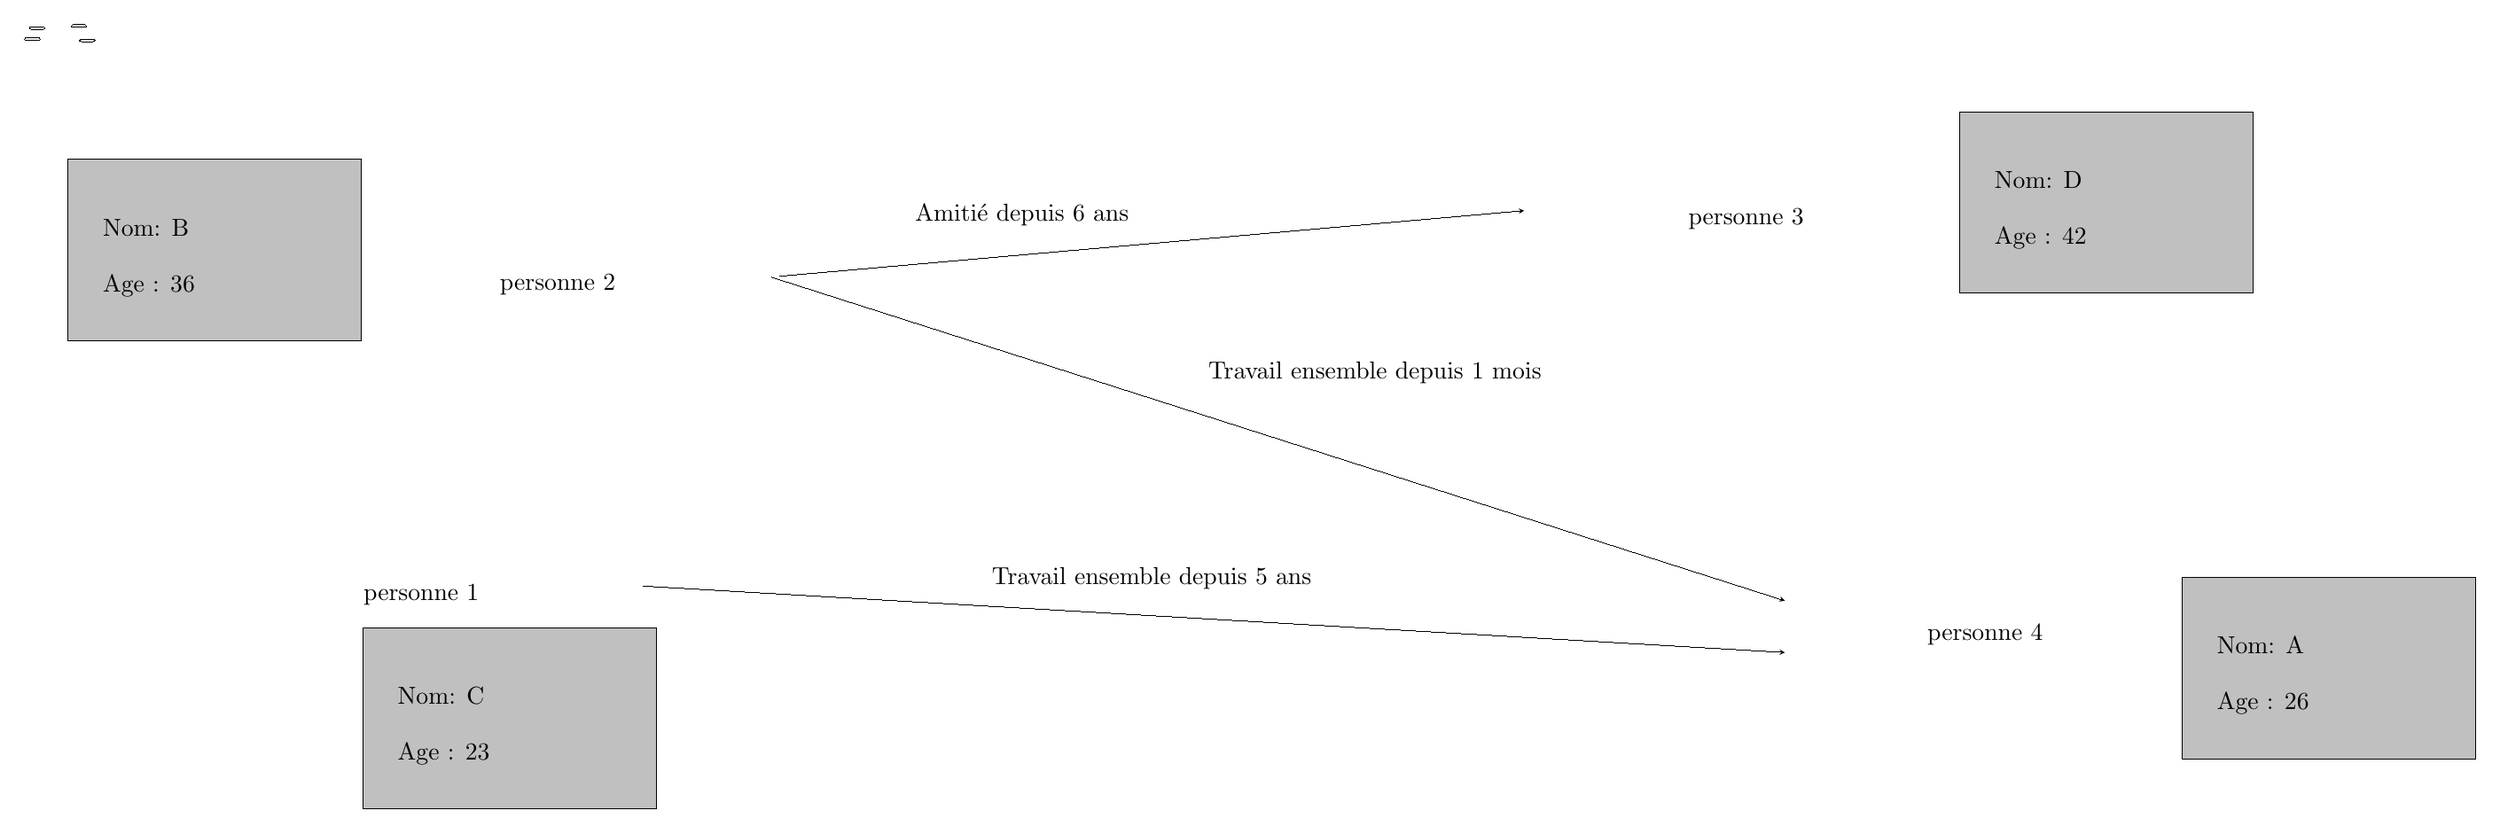
\begin{tikzpicture}[even odd rule]
\pgftransformxscale{1.000000}
\pgftransformyscale{-1.000000}
\definecolor{dialinecolor}{rgb}{0.000000, 0.000000, 0.000000}
\pgfsetstrokecolor{dialinecolor}
\pgfsetstrokeopacity{1.000000}
\definecolor{diafillcolor}{rgb}{1.000000, 1.000000, 1.000000}
\pgfsetfillcolor{diafillcolor}
\pgfsetfillopacity{1.000000}
\pgfsetlinewidth{0.000000\du}
\pgfsetdash{}{0pt}
\pgfsetbuttcap
\pgfsetmiterjoin
\pgfsetlinewidth{0.000000\du}
\pgfsetbuttcap
\pgfsetmiterjoin
\pgfsetdash{}{0pt}
\definecolor{diafillcolor}{rgb}{0.960784, 0.960784, 0.960784}
\pgfsetfillcolor{diafillcolor}
\pgfsetfillopacity{1.000000}
\definecolor{dialinecolor}{rgb}{0.000000, 0.000000, 0.000000}
\pgfsetstrokecolor{dialinecolor}
\pgfsetstrokeopacity{1.000000}
\pgfpathmoveto{\pgfpoint{3.655000\du}{7.600000\du}}
\pgfpathlineto{\pgfpoint{7.895000\du}{7.600000\du}}
\pgfpathcurveto{\pgfpoint{8.480422\du}{7.600000\du}}{\pgfpoint{8.955000\du}{7.835050\du}}{\pgfpoint{8.955000\du}{8.125000\du}}
\pgfpathcurveto{\pgfpoint{8.955000\du}{8.414950\du}}{\pgfpoint{8.480422\du}{8.650000\du}}{\pgfpoint{7.895000\du}{8.650000\du}}
\pgfpathlineto{\pgfpoint{3.655000\du}{8.650000\du}}
\pgfpathcurveto{\pgfpoint{3.069578\du}{8.650000\du}}{\pgfpoint{2.595000\du}{8.414950\du}}{\pgfpoint{2.595000\du}{8.125000\du}}
\pgfpathcurveto{\pgfpoint{2.595000\du}{7.835050\du}}{\pgfpoint{3.069578\du}{7.600000\du}}{\pgfpoint{3.655000\du}{7.600000\du}}
\pgfpathclose
\pgfusepath{fill,stroke}
% setfont left to latex
\definecolor{dialinecolor}{rgb}{0.000000, 0.000000, 0.000000}
\pgfsetstrokecolor{dialinecolor}
\pgfsetstrokeopacity{1.000000}
\definecolor{diafillcolor}{rgb}{0.000000, 0.000000, 0.000000}
\pgfsetfillcolor{diafillcolor}
\pgfsetfillopacity{1.000000}
\node[anchor=base,inner sep=0pt, outer sep=0pt,color=dialinecolor] at (5.775000\du,8.325000\du){personne 1};
\pgfsetlinewidth{0.000000\du}
\pgfsetdash{}{0pt}
\pgfsetbuttcap
\pgfsetmiterjoin
\pgfsetlinewidth{0.000000\du}
\pgfsetbuttcap
\pgfsetmiterjoin
\pgfsetdash{}{0pt}
\definecolor{diafillcolor}{rgb}{0.960784, 0.960784, 0.960784}
\pgfsetfillcolor{diafillcolor}
\pgfsetfillopacity{1.000000}
\definecolor{dialinecolor}{rgb}{0.000000, 0.000000, 0.000000}
\pgfsetstrokecolor{dialinecolor}
\pgfsetstrokeopacity{1.000000}
\pgfpathmoveto{\pgfpoint{5.608750\du}{3.160000\du}}
\pgfpathlineto{\pgfpoint{9.848750\du}{3.160000\du}}
\pgfpathcurveto{\pgfpoint{10.434172\du}{3.160000\du}}{\pgfpoint{10.908750\du}{3.395050\du}}{\pgfpoint{10.908750\du}{3.685000\du}}
\pgfpathcurveto{\pgfpoint{10.908750\du}{3.974950\du}}{\pgfpoint{10.434172\du}{4.210000\du}}{\pgfpoint{9.848750\du}{4.210000\du}}
\pgfpathlineto{\pgfpoint{5.608750\du}{4.210000\du}}
\pgfpathcurveto{\pgfpoint{5.023328\du}{4.210000\du}}{\pgfpoint{4.548750\du}{3.974950\du}}{\pgfpoint{4.548750\du}{3.685000\du}}
\pgfpathcurveto{\pgfpoint{4.548750\du}{3.395050\du}}{\pgfpoint{5.023328\du}{3.160000\du}}{\pgfpoint{5.608750\du}{3.160000\du}}
\pgfpathclose
\pgfusepath{fill,stroke}
% setfont left to latex
\definecolor{dialinecolor}{rgb}{0.000000, 0.000000, 0.000000}
\pgfsetstrokecolor{dialinecolor}
\pgfsetstrokeopacity{1.000000}
\definecolor{diafillcolor}{rgb}{0.000000, 0.000000, 0.000000}
\pgfsetfillcolor{diafillcolor}
\pgfsetfillopacity{1.000000}
\node[anchor=base,inner sep=0pt, outer sep=0pt,color=dialinecolor] at (7.728750\du,3.885000\du){personne 2};
\pgfsetlinewidth{0.000000\du}
\pgfsetdash{}{0pt}
\pgfsetbuttcap
\pgfsetmiterjoin
\pgfsetlinewidth{0.000000\du}
\pgfsetbuttcap
\pgfsetmiterjoin
\pgfsetdash{}{0pt}
\definecolor{diafillcolor}{rgb}{0.960784, 0.960784, 0.960784}
\pgfsetfillcolor{diafillcolor}
\pgfsetfillopacity{1.000000}
\definecolor{dialinecolor}{rgb}{0.000000, 0.000000, 0.000000}
\pgfsetstrokecolor{dialinecolor}
\pgfsetstrokeopacity{1.000000}
\pgfpathmoveto{\pgfpoint{22.633750\du}{2.220000\du}}
\pgfpathlineto{\pgfpoint{26.873750\du}{2.220000\du}}
\pgfpathcurveto{\pgfpoint{27.459172\du}{2.220000\du}}{\pgfpoint{27.933750\du}{2.455050\du}}{\pgfpoint{27.933750\du}{2.745000\du}}
\pgfpathcurveto{\pgfpoint{27.933750\du}{3.034950\du}}{\pgfpoint{27.459172\du}{3.270000\du}}{\pgfpoint{26.873750\du}{3.270000\du}}
\pgfpathlineto{\pgfpoint{22.633750\du}{3.270000\du}}
\pgfpathcurveto{\pgfpoint{22.048328\du}{3.270000\du}}{\pgfpoint{21.573750\du}{3.034950\du}}{\pgfpoint{21.573750\du}{2.745000\du}}
\pgfpathcurveto{\pgfpoint{21.573750\du}{2.455050\du}}{\pgfpoint{22.048328\du}{2.220000\du}}{\pgfpoint{22.633750\du}{2.220000\du}}
\pgfpathclose
\pgfusepath{fill,stroke}
% setfont left to latex
\definecolor{dialinecolor}{rgb}{0.000000, 0.000000, 0.000000}
\pgfsetstrokecolor{dialinecolor}
\pgfsetstrokeopacity{1.000000}
\definecolor{diafillcolor}{rgb}{0.000000, 0.000000, 0.000000}
\pgfsetfillcolor{diafillcolor}
\pgfsetfillopacity{1.000000}
\node[anchor=base,inner sep=0pt, outer sep=0pt,color=dialinecolor] at (24.753750\du,2.945000\du){personne 3};
\pgfsetlinewidth{0.000000\du}
\pgfsetdash{}{0pt}
\pgfsetbuttcap
\pgfsetmiterjoin
\pgfsetlinewidth{0.000000\du}
\pgfsetbuttcap
\pgfsetmiterjoin
\pgfsetdash{}{0pt}
\definecolor{diafillcolor}{rgb}{0.960784, 0.960784, 0.960784}
\pgfsetfillcolor{diafillcolor}
\pgfsetfillopacity{1.000000}
\definecolor{dialinecolor}{rgb}{0.000000, 0.000000, 0.000000}
\pgfsetstrokecolor{dialinecolor}
\pgfsetstrokeopacity{1.000000}
\pgfpathmoveto{\pgfpoint{26.058750\du}{8.180000\du}}
\pgfpathlineto{\pgfpoint{30.298750\du}{8.180000\du}}
\pgfpathcurveto{\pgfpoint{30.884172\du}{8.180000\du}}{\pgfpoint{31.358750\du}{8.415050\du}}{\pgfpoint{31.358750\du}{8.705000\du}}
\pgfpathcurveto{\pgfpoint{31.358750\du}{8.994950\du}}{\pgfpoint{30.884172\du}{9.230000\du}}{\pgfpoint{30.298750\du}{9.230000\du}}
\pgfpathlineto{\pgfpoint{26.058750\du}{9.230000\du}}
\pgfpathcurveto{\pgfpoint{25.473328\du}{9.230000\du}}{\pgfpoint{24.998750\du}{8.994950\du}}{\pgfpoint{24.998750\du}{8.705000\du}}
\pgfpathcurveto{\pgfpoint{24.998750\du}{8.415050\du}}{\pgfpoint{25.473328\du}{8.180000\du}}{\pgfpoint{26.058750\du}{8.180000\du}}
\pgfpathclose
\pgfusepath{fill,stroke}
% setfont left to latex
\definecolor{dialinecolor}{rgb}{0.000000, 0.000000, 0.000000}
\pgfsetstrokecolor{dialinecolor}
\pgfsetstrokeopacity{1.000000}
\definecolor{diafillcolor}{rgb}{0.000000, 0.000000, 0.000000}
\pgfsetfillcolor{diafillcolor}
\pgfsetfillopacity{1.000000}
\node[anchor=base,inner sep=0pt, outer sep=0pt,color=dialinecolor] at (28.178750\du,8.905000\du){personne 4};
\pgfsetlinewidth{0.000000\du}
\pgfsetdash{}{0pt}
\pgfsetbuttcap
{
\definecolor{diafillcolor}{rgb}{0.000000, 0.000000, 0.000000}
\pgfsetfillcolor{diafillcolor}
\pgfsetfillopacity{1.000000}
% was here!!!
\pgfsetarrowsend{stealth}
\definecolor{dialinecolor}{rgb}{0.000000, 0.000000, 0.000000}
\pgfsetstrokecolor{dialinecolor}
\pgfsetstrokeopacity{1.000000}
\draw (10.908750\du,3.685000\du)--(21.573750\du,2.745000\du);
}
% setfont left to latex
\definecolor{dialinecolor}{rgb}{0.000000, 0.000000, 0.000000}
\pgfsetstrokecolor{dialinecolor}
\pgfsetstrokeopacity{1.000000}
\definecolor{diafillcolor}{rgb}{0.000000, 0.000000, 0.000000}
\pgfsetfillcolor{diafillcolor}
\pgfsetfillopacity{1.000000}
\node[anchor=base west,inner sep=0pt,outer sep=0pt,color=dialinecolor] at (12.850000\du,2.900000\du){Amitié depuis 6 ans};
\pgfsetlinewidth{0.000000\du}
\pgfsetdash{}{0pt}
\pgfsetbuttcap
{
\definecolor{diafillcolor}{rgb}{0.000000, 0.000000, 0.000000}
\pgfsetfillcolor{diafillcolor}
\pgfsetfillopacity{1.000000}
% was here!!!
\pgfsetarrowsend{stealth}
\definecolor{dialinecolor}{rgb}{0.000000, 0.000000, 0.000000}
\pgfsetstrokecolor{dialinecolor}
\pgfsetstrokeopacity{1.000000}
\draw (8.955000\du,8.125000\du)--(25.309224\du,9.076227\du);
}
% setfont left to latex
\definecolor{dialinecolor}{rgb}{0.000000, 0.000000, 0.000000}
\pgfsetstrokecolor{dialinecolor}
\pgfsetstrokeopacity{1.000000}
\definecolor{diafillcolor}{rgb}{0.000000, 0.000000, 0.000000}
\pgfsetfillcolor{diafillcolor}
\pgfsetfillopacity{1.000000}
\node[anchor=base west,inner sep=0pt,outer sep=0pt,color=dialinecolor] at (13.950000\du,8.100000\du){Travail ensemble depuis 5 ans};
\pgfsetlinewidth{0.000000\du}
\pgfsetdash{}{0pt}
\pgfsetbuttcap
{
\definecolor{diafillcolor}{rgb}{0.000000, 0.000000, 0.000000}
\pgfsetfillcolor{diafillcolor}
\pgfsetfillopacity{1.000000}
% was here!!!
\pgfsetarrowsend{stealth}
\definecolor{dialinecolor}{rgb}{0.000000, 0.000000, 0.000000}
\pgfsetstrokecolor{dialinecolor}
\pgfsetstrokeopacity{1.000000}
\draw (10.800000\du,3.700000\du)--(25.309224\du,8.333773\du);
}
% setfont left to latex
\definecolor{dialinecolor}{rgb}{0.000000, 0.000000, 0.000000}
\pgfsetstrokecolor{dialinecolor}
\pgfsetstrokeopacity{1.000000}
\definecolor{diafillcolor}{rgb}{0.000000, 0.000000, 0.000000}
\pgfsetfillcolor{diafillcolor}
\pgfsetfillopacity{1.000000}
\node[anchor=base west,inner sep=0pt,outer sep=0pt,color=dialinecolor] at (17.050000\du,5.150000\du){Travail ensemble depuis 1 mois};
\pgfsetlinewidth{0.000000\du}
\pgfsetdash{}{0pt}
\pgfsetmiterjoin
{\pgfsetcornersarced{\pgfpoint{0.000000\du}{0.000000\du}}\definecolor{diafillcolor}{rgb}{0.752941, 0.752941, 0.752941}
\pgfsetfillcolor{diafillcolor}
\pgfsetfillopacity{1.000000}
\fill (31.000050\du,8.000000\du)--(31.000050\du,10.600000\du)--(35.200050\du,10.600000\du)--(35.200050\du,8.000000\du)--cycle;
}{\pgfsetcornersarced{\pgfpoint{0.000000\du}{0.000000\du}}\definecolor{dialinecolor}{rgb}{0.000000, 0.000000, 0.000000}
\pgfsetstrokecolor{dialinecolor}
\pgfsetstrokeopacity{1.000000}
\draw (31.000050\du,8.000000\du)--(31.000050\du,10.600000\du)--(35.200050\du,10.600000\du)--(35.200050\du,8.000000\du)--cycle;
}% setfont left to latex
\definecolor{dialinecolor}{rgb}{0.000000, 0.000000, 0.000000}
\pgfsetstrokecolor{dialinecolor}
\pgfsetstrokeopacity{1.000000}
\definecolor{diafillcolor}{rgb}{0.000000, 0.000000, 0.000000}
\pgfsetfillcolor{diafillcolor}
\pgfsetfillopacity{1.000000}
\node[anchor=base west,inner sep=0pt,outer sep=0pt,color=dialinecolor] at (31.500050\du,9.095000\du){Nom: A};
% setfont left to latex
\definecolor{dialinecolor}{rgb}{0.000000, 0.000000, 0.000000}
\pgfsetstrokecolor{dialinecolor}
\pgfsetstrokeopacity{1.000000}
\definecolor{diafillcolor}{rgb}{0.000000, 0.000000, 0.000000}
\pgfsetfillcolor{diafillcolor}
\pgfsetfillopacity{1.000000}
\node[anchor=base west,inner sep=0pt,outer sep=0pt,color=dialinecolor] at (31.500050\du,9.895000\du){Age : 26 };
\pgfsetlinewidth{0.000000\du}
\pgfsetdash{}{0pt}
\pgfsetmiterjoin
{\pgfsetcornersarced{\pgfpoint{0.000000\du}{0.000000\du}}\definecolor{diafillcolor}{rgb}{0.752941, 0.752941, 0.752941}
\pgfsetfillcolor{diafillcolor}
\pgfsetfillopacity{1.000000}
\fill (0.713750\du,2.010000\du)--(0.713750\du,4.610000\du)--(4.913750\du,4.610000\du)--(4.913750\du,2.010000\du)--cycle;
}{\pgfsetcornersarced{\pgfpoint{0.000000\du}{0.000000\du}}\definecolor{dialinecolor}{rgb}{0.000000, 0.000000, 0.000000}
\pgfsetstrokecolor{dialinecolor}
\pgfsetstrokeopacity{1.000000}
\draw (0.713750\du,2.010000\du)--(0.713750\du,4.610000\du)--(4.913750\du,4.610000\du)--(4.913750\du,2.010000\du)--cycle;
}% setfont left to latex
\definecolor{dialinecolor}{rgb}{0.000000, 0.000000, 0.000000}
\pgfsetstrokecolor{dialinecolor}
\pgfsetstrokeopacity{1.000000}
\definecolor{diafillcolor}{rgb}{0.000000, 0.000000, 0.000000}
\pgfsetfillcolor{diafillcolor}
\pgfsetfillopacity{1.000000}
\node[anchor=base west,inner sep=0pt,outer sep=0pt,color=dialinecolor] at (1.213750\du,3.105000\du){Nom: B};
% setfont left to latex
\definecolor{dialinecolor}{rgb}{0.000000, 0.000000, 0.000000}
\pgfsetstrokecolor{dialinecolor}
\pgfsetstrokeopacity{1.000000}
\definecolor{diafillcolor}{rgb}{0.000000, 0.000000, 0.000000}
\pgfsetfillcolor{diafillcolor}
\pgfsetfillopacity{1.000000}
\node[anchor=base west,inner sep=0pt,outer sep=0pt,color=dialinecolor] at (1.213750\du,3.905000\du){Age : 36 };
\pgfsetlinewidth{0.000000\du}
\pgfsetdash{}{0pt}
\pgfsetmiterjoin
{\pgfsetcornersarced{\pgfpoint{0.000000\du}{0.000000\du}}\definecolor{diafillcolor}{rgb}{0.752941, 0.752941, 0.752941}
\pgfsetfillcolor{diafillcolor}
\pgfsetfillopacity{1.000000}
\fill (4.938750\du,8.720000\du)--(4.938750\du,11.320000\du)--(9.138750\du,11.320000\du)--(9.138750\du,8.720000\du)--cycle;
}{\pgfsetcornersarced{\pgfpoint{0.000000\du}{0.000000\du}}\definecolor{dialinecolor}{rgb}{0.000000, 0.000000, 0.000000}
\pgfsetstrokecolor{dialinecolor}
\pgfsetstrokeopacity{1.000000}
\draw (4.938750\du,8.720000\du)--(4.938750\du,11.320000\du)--(9.138750\du,11.320000\du)--(9.138750\du,8.720000\du)--cycle;
}% setfont left to latex
\definecolor{dialinecolor}{rgb}{0.000000, 0.000000, 0.000000}
\pgfsetstrokecolor{dialinecolor}
\pgfsetstrokeopacity{1.000000}
\definecolor{diafillcolor}{rgb}{0.000000, 0.000000, 0.000000}
\pgfsetfillcolor{diafillcolor}
\pgfsetfillopacity{1.000000}
\node[anchor=base west,inner sep=0pt,outer sep=0pt,color=dialinecolor] at (5.438750\du,9.815000\du){Nom: C};
% setfont left to latex
\definecolor{dialinecolor}{rgb}{0.000000, 0.000000, 0.000000}
\pgfsetstrokecolor{dialinecolor}
\pgfsetstrokeopacity{1.000000}
\definecolor{diafillcolor}{rgb}{0.000000, 0.000000, 0.000000}
\pgfsetfillcolor{diafillcolor}
\pgfsetfillopacity{1.000000}
\node[anchor=base west,inner sep=0pt,outer sep=0pt,color=dialinecolor] at (5.438750\du,10.615000\du){Age : 23 };
\pgfsetlinewidth{0.000000\du}
\pgfsetdash{}{0pt}
\pgfsetmiterjoin
{\pgfsetcornersarced{\pgfpoint{0.000000\du}{0.000000\du}}\definecolor{diafillcolor}{rgb}{0.752941, 0.752941, 0.752941}
\pgfsetfillcolor{diafillcolor}
\pgfsetfillopacity{1.000000}
\fill (27.813750\du,1.330000\du)--(27.813750\du,3.930000\du)--(32.013750\du,3.930000\du)--(32.013750\du,1.330000\du)--cycle;
}{\pgfsetcornersarced{\pgfpoint{0.000000\du}{0.000000\du}}\definecolor{dialinecolor}{rgb}{0.000000, 0.000000, 0.000000}
\pgfsetstrokecolor{dialinecolor}
\pgfsetstrokeopacity{1.000000}
\draw (27.813750\du,1.330000\du)--(27.813750\du,3.930000\du)--(32.013750\du,3.930000\du)--(32.013750\du,1.330000\du)--cycle;
}% setfont left to latex
\definecolor{dialinecolor}{rgb}{0.000000, 0.000000, 0.000000}
\pgfsetstrokecolor{dialinecolor}
\pgfsetstrokeopacity{1.000000}
\definecolor{diafillcolor}{rgb}{0.000000, 0.000000, 0.000000}
\pgfsetfillcolor{diafillcolor}
\pgfsetfillopacity{1.000000}
\node[anchor=base west,inner sep=0pt,outer sep=0pt,color=dialinecolor] at (28.313750\du,2.425000\du){Nom: D};
% setfont left to latex
\definecolor{dialinecolor}{rgb}{0.000000, 0.000000, 0.000000}
\pgfsetstrokecolor{dialinecolor}
\pgfsetstrokeopacity{1.000000}
\definecolor{diafillcolor}{rgb}{0.000000, 0.000000, 0.000000}
\pgfsetfillcolor{diafillcolor}
\pgfsetfillopacity{1.000000}
\node[anchor=base west,inner sep=0pt,outer sep=0pt,color=dialinecolor] at (28.313750\du,3.225000\du){Age : 42 };
\end{tikzpicture}

	    }
		\caption{Illustration d'une base de données NoSQL de type graphe}
		\label{fig:graphe-nosql}
	\end{figure}
	
	Il existe plusieurs implémentations des quatre types de bases de données. Chaque implémentation favorise un ou plus des éléments suivants : la disponibilité des données, la cohérence des données et la tolérance au partitionnement.  C'est ce qu'explique le théorème CAP.	
		
		\paragraph{Big Data et le théorème  CAP} \label{par:cap-theorem}:
		
		Le théorème CAP annonce que dans le cadre d'un système distribué où les données sont réparties sur plusieurs machines (ou n\oe{}uds),
		%(ou n\oe{}uds) (voir \ref{sec:distruted-camput}),  
		une base de données ne peut pas garantir les trois attributs suivants: \textit{Consistency}, \textit{Availability}, et \textit{Partition Tolerence}  en même temps. 
		
		
			\subparagraph{ Consistency (ou intégrité)} Chaque donnée a un seul état visible depuis l'extérieur. Par exemple, les différents serveurs hébergeant la base de données voient tous les mêmes données. Ainsi, une lecture faite après une écriture doit renvoyer la donnée précédemment écrite;
			
			\subparagraph{ Availability (ou disponibilité)} Une base de données doit toujours fournir une réponse à une requête d'un client; 
			
			%En cas d'une panne technique sur un des serveurs qui hébergent  la base de données, il faut s'assurer de desservir  des clients.  Généralement, cela est assuré à travers la réplication des données
			
			 \subparagraph{Partition tolerance (ou la tolérance au partitionnement) } Une coupure du réseau entre deux n\oe{}uds ou l'indisponibilité d'un de ces n\oe{}uds ne devrait pas affecter le bon fonctionnement du système. Tout de même,  ce dernier doit répondre à la demande d'un client. 

		
		%conclusion
		Les trois attributs du théorème CAP s'opposent entre eux. On distingue les trois scénarios possibles:
		
		\begin{itemize}
			\item [--] Le couple \textbf{CA} : les SGBDR adoptent les deux attributs C et A, qui sont une forte cohérence et disponibilité. Cependant, l'attribut partitionnement réseau n'est pas toujours pris en compte.
			\item [--] Le couple \textbf{CP} : les implémentations du C et du P assurent la tolérance aux pannes en distribuant les données sur plusieurs serveurs. Malgré cette réplication, ces implémentations assurent la cohérence des données même en présence de mises à jour concurrentielles.
			\item [--] Le couple \textbf{AP} : les implémentations du A et du  P assurent un temps de réponse rapide et une réplication des données. Cependant, les mises à jour étant asynchrones, la garantie que la version d'une donnée soit bonne, ne peut pas être assurée.
			
		\end{itemize}
		
		La figure \ref{fig:cap} présente des implémentations des différents types de bases de données NoSQL pour chaque couple CA, CP et AP.
		
		\begin{figure}[H]
			\centering
			\captionsetup{justification=centering}
			\includegraphics[width=1\linewidth]{illustrations/cap}
			\caption{Bases de données NoSQL suivant le théorème de CAP }
			\label{fig:cap}
			\source{\url{https://payberah.github.io/files/download/p2p/nosql.pdf}, consultée le $05/08/2018$.}
		\end{figure}
		
		
		
		Le choix d'une base de données relationnelle ou NoSQL dépend des besoins des entreprises. En terme de tendances, la figure \ref{fig:ranking-db} reprend un classement des SGBDs au $1$ août $ 2018 $. La suite de la liste ainsi que  la méthode qui dirige ce classement sont    disponibles sur le site  web \textit{DB-Engines Ranking}\footnote{Source : \url{https://db-engines.com/},  consultée le $01/08/2018$.}. Parmi les critères de classement, on trouve le nombre de références du SGBD sur les sites Internet. 
		
		%Ce nombre de référence est quantifiable à partir du  nombre lui-même de résultats obtenus des différents moteurs de recherche comme Google, Bing, etc. 
		
		\begin{figure}[H]
			\centering
			\captionsetup{justification=centering}
			\includegraphics[width=1\linewidth]{illustrations/ranking-db}
			\caption{Un classement des SGBDs sur \textit{DB-Engines Ranking} du $1$ août $2018$ }
			\label{fig:ranking-db}
			\source{\url{https://db-engines.com/en/ranking}, consultée le $01/08/2018$.}
		\end{figure}
		
		
		
		\subsection{Schema on Write VS Schema on Read} \label{sec:schema-read-write}
		
		Lors du chargement des données depuis leurs sources de stockage pour tout type de manipulation, on distingue deux approches : \textit{ Schema on Write} et \textit{Schema on Read}.
		% L'approche \textit{Schema on Read } est celle utilisée par l'outil Amazon Athena présenté dans la section \ref{par:allservices}.
		
		Dans la première, il faut définir les colonnes, le format de données, les types, etc. La lecture des données est rapide et moins coûteuse étant donné l'effort entreprit pour définir la structure. C'est le cas des bases de données relationnelles.
		
		Dans la deuxième, les données sont chargées telles qu'elles sont, sans transformations ou changements. L'interprétation de ces données se fait lors de la lecture, et cela dépend des besoins pour lesquels les données sont analysées. Ainsi, les mêmes données peuvent être lues de différentes manières. Par exemple, l'action  de lire les données  d'une colonne, qu'elles soient de type entier ou bien chaîne de caractère d'un fichier CSV est la même, mais le type de la donnée qui diffère.
		
		 Les figures \ref{fig:on-write} et \ref{fig:on-read} illustrent la différence entre ces deux approches.
		\begin{figure}[H]
			\centering
			\includegraphics[width=0.8\linewidth]{illustrations/on-write}
			\caption{Schema on Write (Traditionnelle)}
			\label{fig:on-write}
		\end{figure}
		\begin{figure}[H]
			\centering
			\captionsetup{justification=centering}
			\includegraphics[width=0.8\linewidth]{illustrations/on-read}
			\caption{Schema on Read (Big Data)}
			\label{fig:on-read}
			\source{ \url{https://blogs.oracle.com/datawarehousing/big-data-sql-quick-start-schema-on-read-and-schema-on-write-part11}, consultée le $05/08/2018$.}
		\end{figure}
		
		La meilleure approche dépend des besoins de l'analyse. La première approche est meilleure en performances, cependant, la deuxième est tolérante aux erreurs  humaines.
		
		
		\subsection{L'informatique distribuée et l'analyse de données massives} \label{sec:distruted-camput}
		Il existe deux stratégies pour appliquer des traitements sur un grand ensemble de données: 
		
		
		\begin{itemize}
			\item[--] Par distribution des traitements (\textit{scaling} des traitements)~: les traitements sont distribués sur un nombre de n\oe{}uds important. De ce fait, les données sont amenées jusqu'à ces n\oe{}uds;
			
			\item[--] Par distribution des données (\textit{scaling} des données)~: les données sont distribuées sur un nombre important de n\oe{}uds. De plus, cela permet  de stocker un maximum de données. Il s'agit d'amener les traitements aux machines sur lesquelles les données sont stockées. Du fait que le stockage de données est réparti sur plusieurs machines, il est possible de traiter des données très volumineuses. La première mise en \oe{}uvre de cette approche est le schéma Map-Reduce. 
		\end{itemize}
	\section{Parcours de quelques technologies du Big Data}
	
